\section{Data description}
The dataset contains a training subset (13538 recordings from 35 sensors), and validation subset (4308 recordings from 9 sensors), and a test subset (669 recordings from 48 sensors). Each recording has been annotated using a set of 23 “tags” like “engine presence, machinery presence, non-machinery-impact presence, dog-barking-whining presence” ~\cite{4}.

The audio files used were recorded using the SONYC acoustic sensor network for monitoring urban noise pollution. In New York City, over 60 distinct sensors have been placed accumulating the equivalent of more than 50 years of audio data, of which a small fraction was used. The data was sampled by picking the closest neighbors based on VGGish qualities of recordings with recognized classes of interest. All of the recordings are 10 seconds long and were made with the same microphones and gain settings. 

The training, validation, and test subsets of the annotation data are contained in annotations.csv. Each row in the file represents one multi-label annotation of a recording—it might be a single citizen science volunteer's annotation, a single SONYC team member's annotation, or the SONYC team's agreed-upon ground truth (for more information, see the annotator id column description).

The sensors in the test set will not disjoint from the training and validation subsets, but the test recordings are displaced in time, occurring after any of the recordings in the training and validation subset. We plan to use the test data to find out the aggregate of mismatch by using a Multi Label classification Machine Learning Model

	
	\begin{figure}[h!]
		
		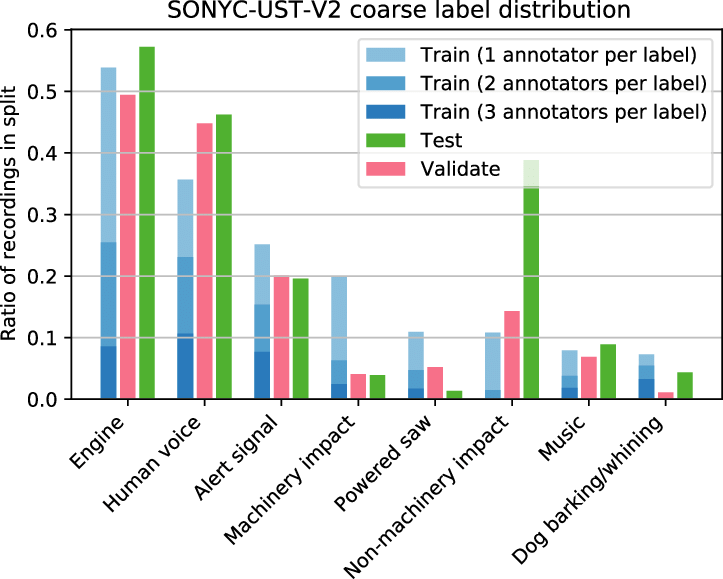
\includegraphics[width=9cm]{figure1}
		\caption{ Classes distibution in data}
	\end{figure}
	


	
	
	
	

	
	